\Chapter{Introduction to Neutrino}
\label{Ch1}

    Neutrinos are leptons carrying neutral electrical charge.
    Its neutral lepton nature makes it a fermion only interact with other particle through electroweak interactions.
    Neutrino was long assumed as mass less particle until the discovery neutrino oscillation, proving neutrino being massive.
    Through decades of study, it is known that neutrino has three flavors and its antiparticle.
    The measurements of neutrino oscillation also found the mass eigenstates are not orthogonal with neutrino flavors, but are significantly mixed with neutrino flavors, compared to quark mixing.
    
    Although many theoretical and experimental efforts involved with neutrino has been put in the history, the discovery and measurements of neutrino only brought more experimental tasks: the absolute mass measurement of neutrino, the observation of lepton CP-violation through neutrino oscillation, probing neutrino-less double beta decay, and  search for sterile neutrino.
    
    Thank to its rare reaction with other particles, neutrino detection has been applied to aid the research of nuclear and astrophysics.
    Reactor antineutrino detector is able to remotely monitor a fission reactors nuclear structure~\cite{bib:DYBSpectrum, bib:DYBEvo}. 
    The neutrino observatory has taken part of the multi-messenger astrophysics observation~\cite{bib:IceCube}.

\Section{Beta-decay}
\label{Ch1Sec2}
    
    The study of neutrino physics began with studies of $\beta$-decay.
    During the early research of radioactive decay, the process of $\beta$-decay was assumed as
    \begin{equation}
    (A, Z) \rightarrow (A, Z+1) + e^-.
    \end{equation}
    With energy and momentum conservation, one can easily conclude that reaction produces $\beta$ with single kinetic energy.
    In 1914, Chadwick found the energy spectrum of $\beta$ particle produced from radioactive decay was continuous~\cite{bib:Chadwick}, different from the $\alpha$ and $\gamma$ products that are sharp distribution.
    Particularly, Ellis and Wooster established the proof of continuous $\beta$ spectrum measurement of $^{210}$Bi~\cite{bib:EandW} shown in Figure~\ref{fig:BiSpectrum}.
    To aid the conservation of energy, in 1932, Pauli postulated neutrino in his ``open letter to the group of radioactive people at the Gauverein meeting in Tübingen", by calling it \textit{``neutron"}, as an additional neutral spin-$\frac{1}{2}$ particle produced in $\beta$-decay.

\begin{figure}[h!]
\centering
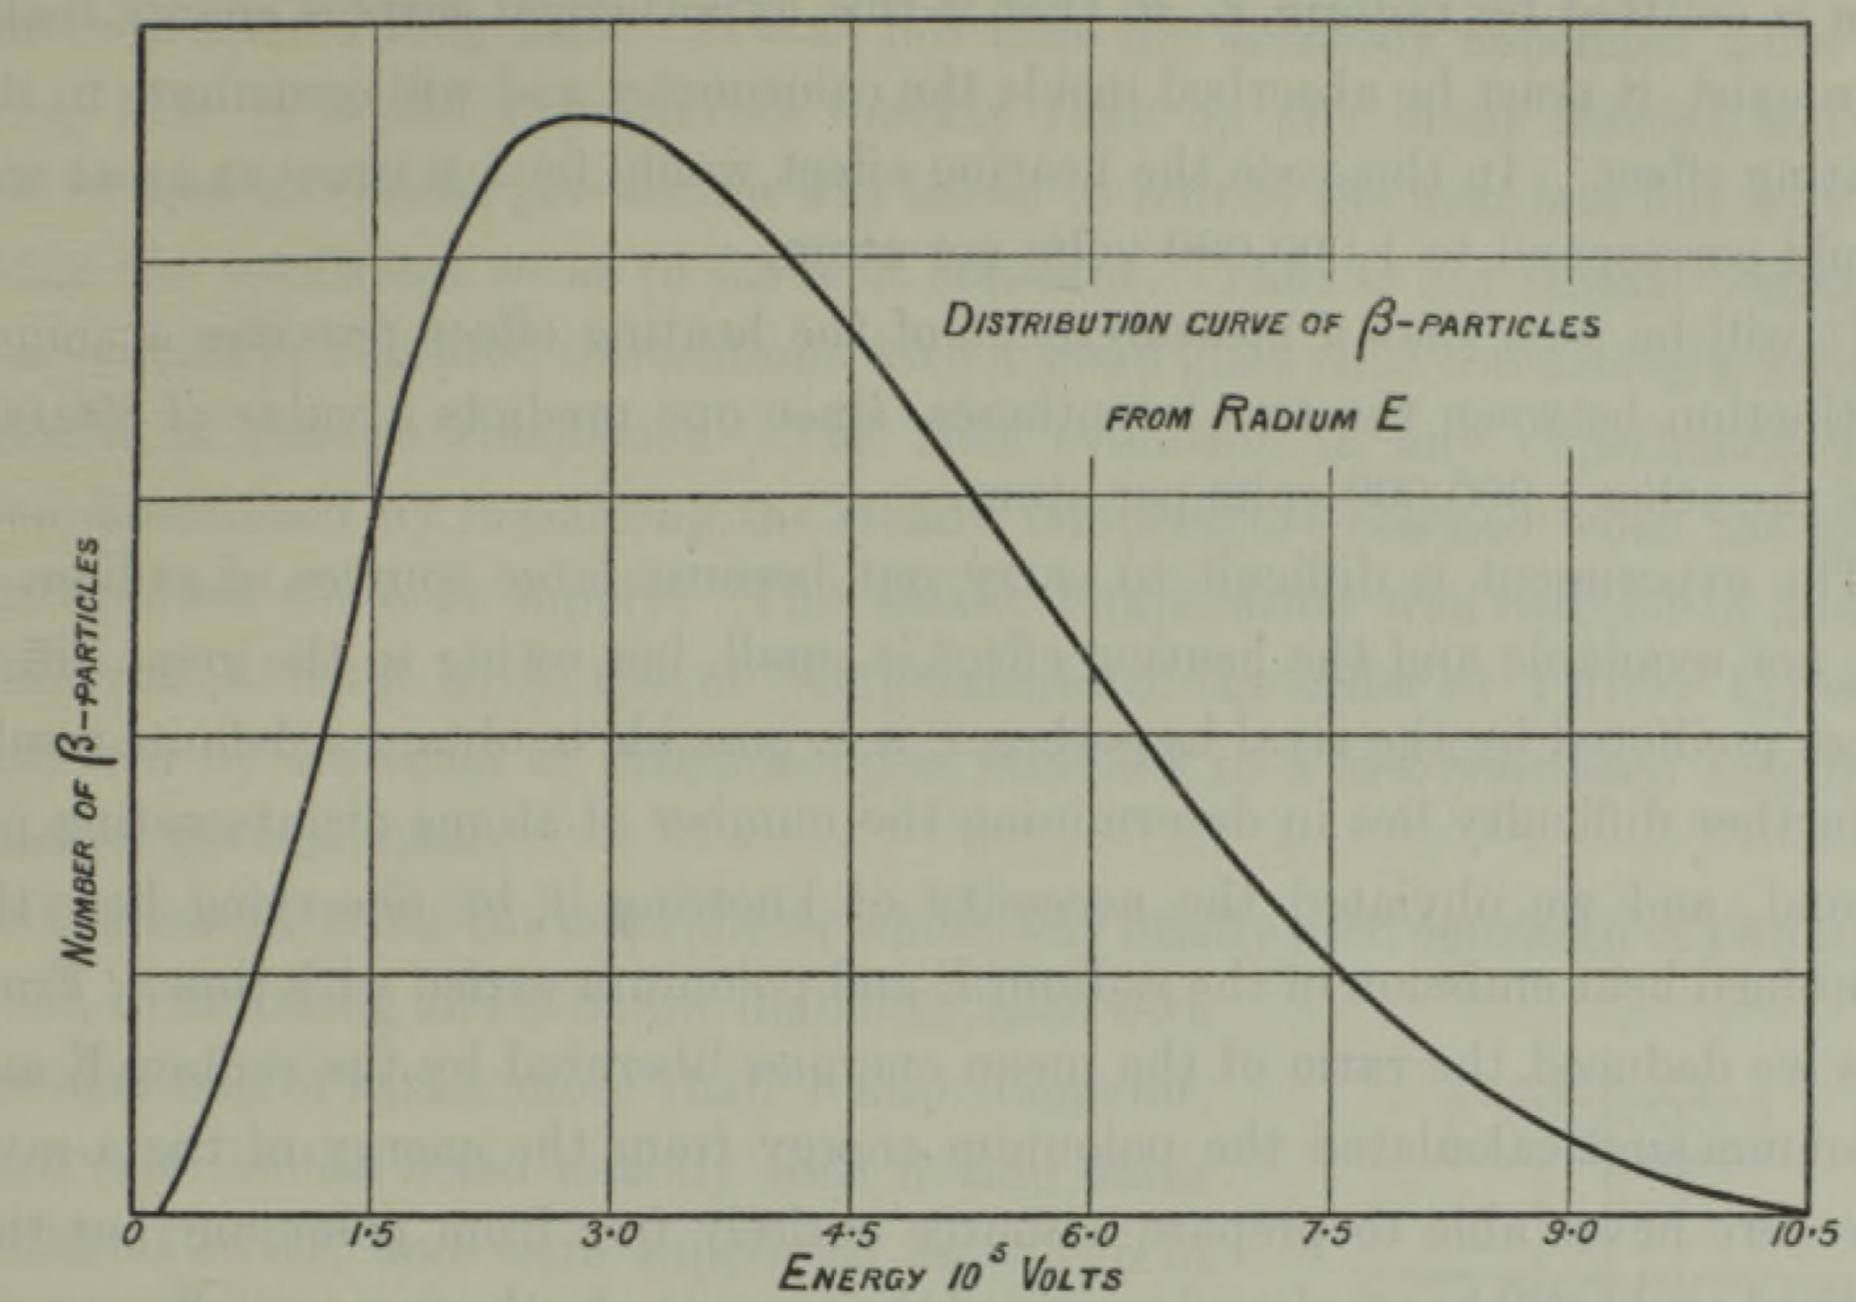
\includegraphics[width=0.6\textwidth]{Figures/BiSpectrum.png}
\caption[Continuous beta spectrum]{The continuous $\beta$ energy spectrum measured from $^{210}$Bi $\beta$-decay~\cite{bib:EandW}.}
\label{fig:BiSpectrum}
\end{figure}    
    
    Soon after the discovery of neutron, Fermi developed his theory of beta decay in 1934~\cite{bib:Fermi}, where the weak interaction was theorized. 
    In Fermi's theory of beta decay, neutrino was incorporated as a massless daughter particle that carries away part of the energy of a neutron beta decay:
    \begin{equation}\label{eq1.1}
        n \rightarrow p + e^- + \nu,
    \end{equation}
    where $\nu$ was named as neutrino for the first time.
    The neutrino generated in this process was later found to be \nuebar (electron antineutrino) to conserve lepton number in this process.

\Section{The Discovery of Neutrinos}
\label{Ch1Sec2}

    Though Pauli, when proposed neutrino's existence, stated it was a particle that \textit{cannot be detected}.
    The discovery of weak interaction found neutrino can interact with other particles by exchanging W or Z bosons.
    Among many types of neutrino-nucleon and -lepton interaction, neutrino can interact the similar way it is generated in $\beta$-decay:
    \begin{equation}
        \label{eq:IBD}
        \nuebar + p \rightarrow n + e^+,
    \end{equation}
    which is named as inverse beta decay (IBD), a quasielastic charged-current reaction between \nuebar and proton by exchanging a W boson.
    The cross-section of IBD reaction is estimated in the order of $\sim 10^{-43}\frac{p_eE_e}{\text{MeV}^2}$~(cm$^2$)~\cite{bib:IBDXsection}, where $p_e$ and $E_e$ are momentum and energy of positron produced.
    Such a rare interaction rate brought great challenge in neutrino detection that requires both high neutrino production from the source and huge amount of proton in the detector.
    
    In 1956, Cowan and Reines discovered neutrino through the detection of IBD~\cite{bib:CowanReines}.
    The neutrinos detected was \nuebar produced from the $\beta$-decay of daughter isotopes of the nuclear fission reactor at Savannah River plant.
    To detect the IBD signals, two target tanks filled with $^{108}$Cd loaded water were deployed in the two gaps made by three vertically aligned liquid scintillator (LS) detector.
    The signature of IBD process was the time coincidence between the positron and neutron produced in the reaction.
    When a proton in the water tank is hit by \nuebar, the produced positron will annihilate into a pair of 0.511~MeV $\gamma$, and the neutron is largely captured by $^{108}$Cd within 5~\textmu s, emitting reactor $\gamma$s with total energy from 3~MeV to 10~MeV.
    The $\gamma$s in the LS generate scintillation photons that are eventually collected by the 110 photomultiplier tubes (PMTs) in each LS detector. 
    By detecting $\gamma$ ray from the target tanks with time coincidence, the Cowan and Reines experiment collected 1013 \nuebar events in 900~hours reactor-on data acquisition.
    
    The conservation of lepton number with flavor requires $\beta$-decay only produce \nuebar.
    This conservation also forbids interactions like $\overline{\nu}_\mu + p \rightarrow n + e^+$, meaning ${\nu}_\mu$'s (muon neutrino) nucleon interaction cannot produce electron~\cite{bib:Ponte1959, bib:Schwartz}.
    In 1962, Schwartz, Lederman, and Steinberger induced high energy $\nu_\mu/\overline{\nu}_\mu$ produced from the decay from accelerated $\pi^\pm$~\cite{bib:numuDiscovery}.
    With 10 tons spark chamber consisting of 90 aluminum plates, the experiment at Brookhaven National Laboratory is able to distinguish electron and muon produced from $\nu_\mu/\overline{\nu}_\mu$'s interaction with nucleons. 
    This experiment discovered $\nu_\mu$ by finding only $\mu^\pm$ was detected in the chamber and so distinguished neutrinos with different flavors.
    
    In 2000, the DONUT collaboration at Fermilab discovered $\nu_\tau$ (tau neutrino) mainly decayed from the accelerated $D_s^- \rightarrow \tau^- + \overline{\nu}_\tau$. 
    Since the discovery of $\nu_\tau$, the family of neutrinos in Standard Model has six members $\nu_e$, $\nu_\mu$, $\nu_\tau$, and their antiparticles.
    
\Section{Observation of Neutrino Oscillation}
    
    Fermi also stated the neutrino being either massless or extremely light in his study of $\beta$-decay~\cite{bib:Fermi}.
    Following Yang and Lee's discussion of parity conservation question~\cite{bib:YangLee}, and Wu discovered that weak interaction violates parity symmetry by observing $\beta$ momentum direction preference from the $\beta$-decay of polarized $^{60}$Co~\cite{bib:Wu}.
    The parity violation of $\beta$-decay restricts the neutrino helicity being only left handed (and antineutrino helicity being only right handed).
    Therefore, massless neutrino and antineutrino is seemingly preferred in nature to obey the proper representation of the Lorentz group.
    The Standard Model was built with the assumption of massless neutrino.
    However, the experimental observation of neutrino oscillation proved neutrino having nonzero masses.

    The research of the oscillating neutrino began from the discovery of solar neutrino problem. 
    In 1968, Davis \textit{et al.} organized the solar neutrino experiment aiming to detect $\nu_e$ from nuclear fission reaction in the sun~\cite{bib:davis}.
    This experiment uses a target containing 390000 liters of C$_2$Cl$_4$ in the Homestake mine to detect the appearance of $^{37}$Ar in the $^{37}$Cl($\nu_e$, $e^-$)$^{37}$Ar reaction.
    The solar neutrino problem arose when the measured flux of $\nu_e$ is one third as predicted by the Standard Solar Model.
    In the following decades, more solar neutrino flux measurement, including GALLEX~\cite{bib:GALLEX}, GNO~\cite{bib:GNO}, SAGE~\cite{bib:SAGE}, and Kamiokande~\cite{bib:kamioka1996}, observed less solar $\nu_e$ flux from expectation.
    Also, atmosphere neutrino measurements, the IMB~\cite{bib:IMB} and Kamiokande~\cite{bib:Kamioka1986} experiments, detected fewer atmosphere neutrino from prediction, which is referred as the \textit{atmosphere neutrino anomaly}.
    These deficits to theoretical models provided the experimental hints to neutrino oscillation. 
    
    The observation of neutrino oscillation was first achieved by the Super-K experiment~\cite{bib:SuperK} in 1998. 
    Using a water Cherenkov detector with 50000 tons of pure and 13000 PMTs, the experiment observed the atmosphere $\nu_\mu$ flux difference among a large variety of zenith angle shown in Figure~\ref{fig:SuperK}.
    The difference of atmosphere neutrino flux was caused by a the $\nu_\mu$s oscillated into other flavors when traveling through the earth until being collected in the detector.
    
\begin{figure}[h!]
\centering
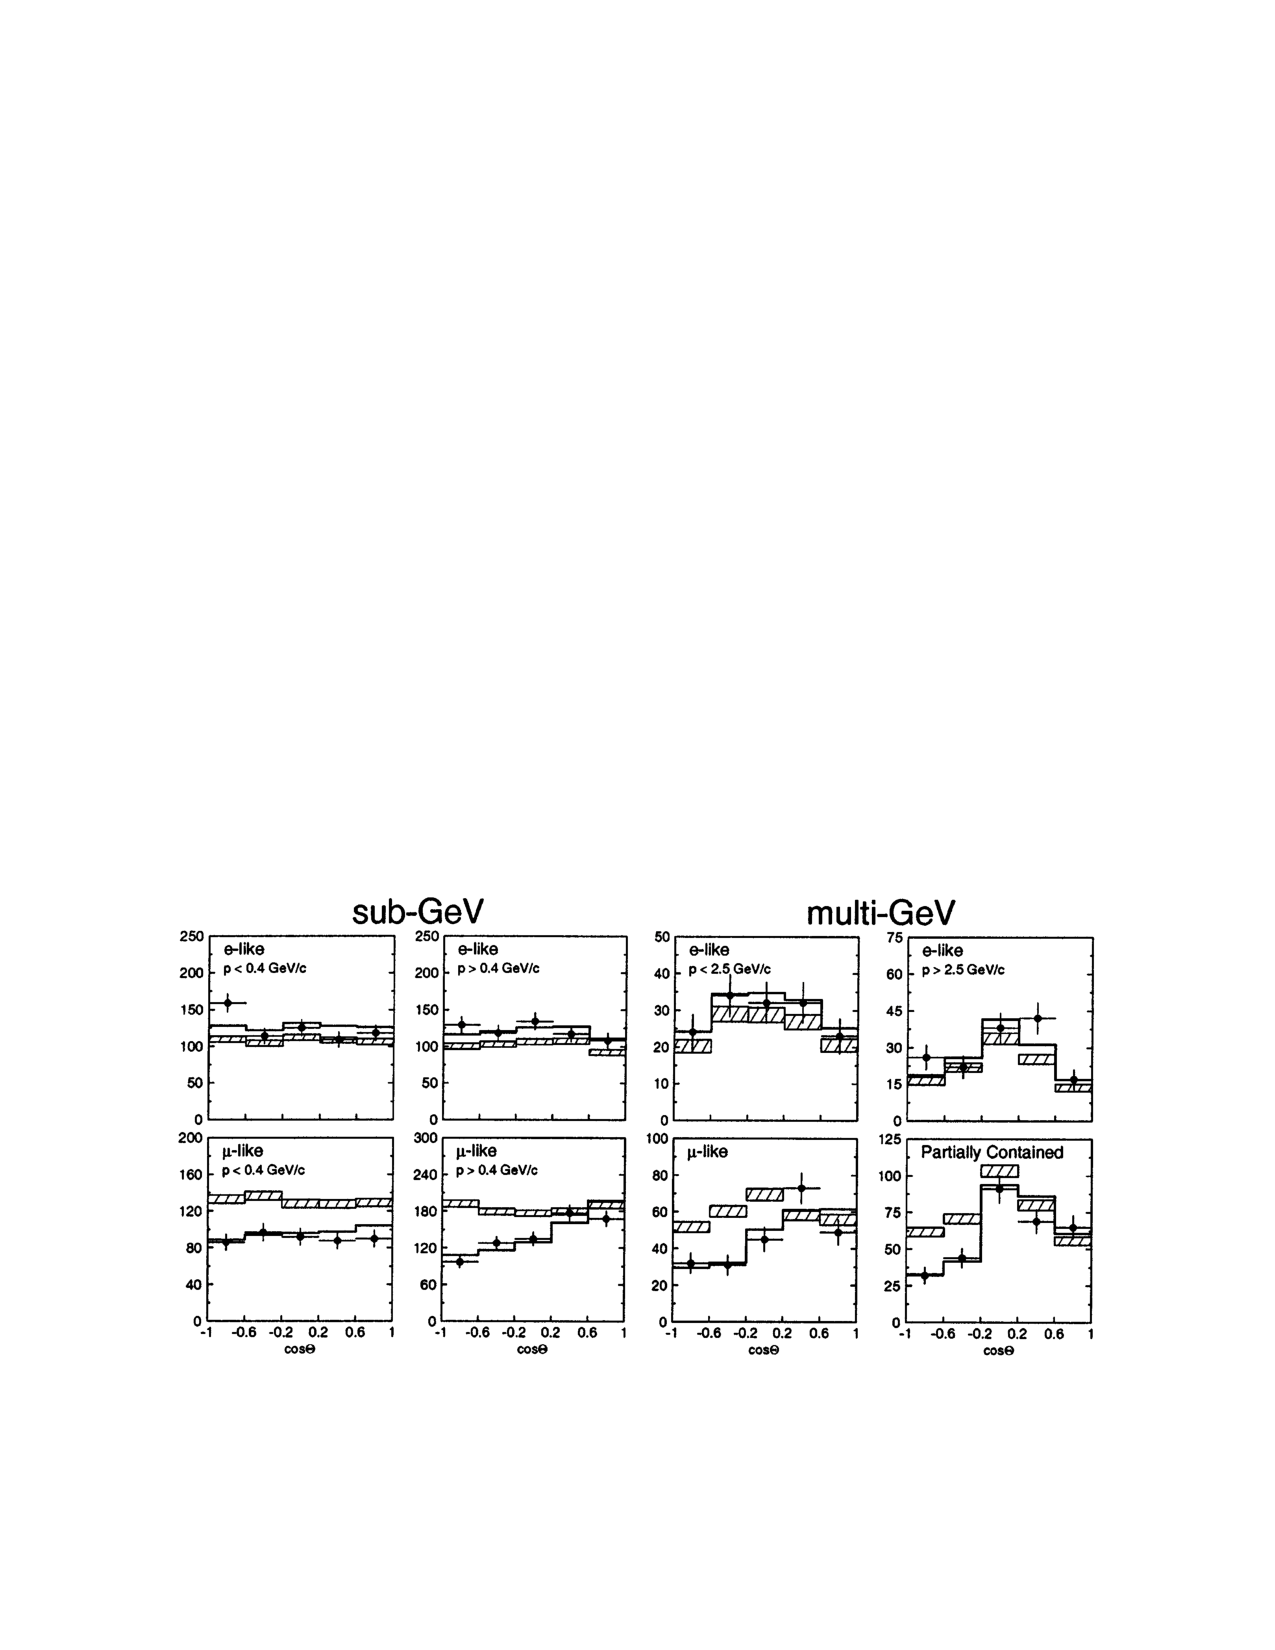
\includegraphics[width=0.95\textwidth]{Figures/SuperK.pdf}
\caption[Atmosphere neutrino oscillation]{The flux of $e$-like and $\mu$-like events measured by the Super-K experiment~\cite{bib:SuperK}. 
The $\mu$-like, correlated to number of $\nu_\mu$ collected, varies significantly with respect to zenith angle. 
The solid line (shaded region) represents the Monte-Carlo (MC) with (without) the model of neutrino oscillation.  }
\label{fig:SuperK}
\end{figure}

    In 2001, SNO experiment~\cite{bib:SNO} deployed heavy water Cherenkov detector that is able to detect charged-current (CC), neutral-current (NC) and elastic scattering (ES) to detect solar neutrinos of all flavors in comparison with $\nu_e$s.
    If neutrino oscillates among flavors, the solar $\nu_e$ will oscillates into other flavors while conserve the  neutrino flux of all flavors.
    As shown in Figure~\ref{fig:sno}, the experiment is able to confirm solar neutrino oscillation by comparing neutrino flux measured with different scattering mode.
    Super-K and SNO experiments provided solid experimental evidences of neutrino oscillation and resolved the solar neutrino problem and atmosphere neutrino anomaly.
    
\begin{figure}[h!]
\centering
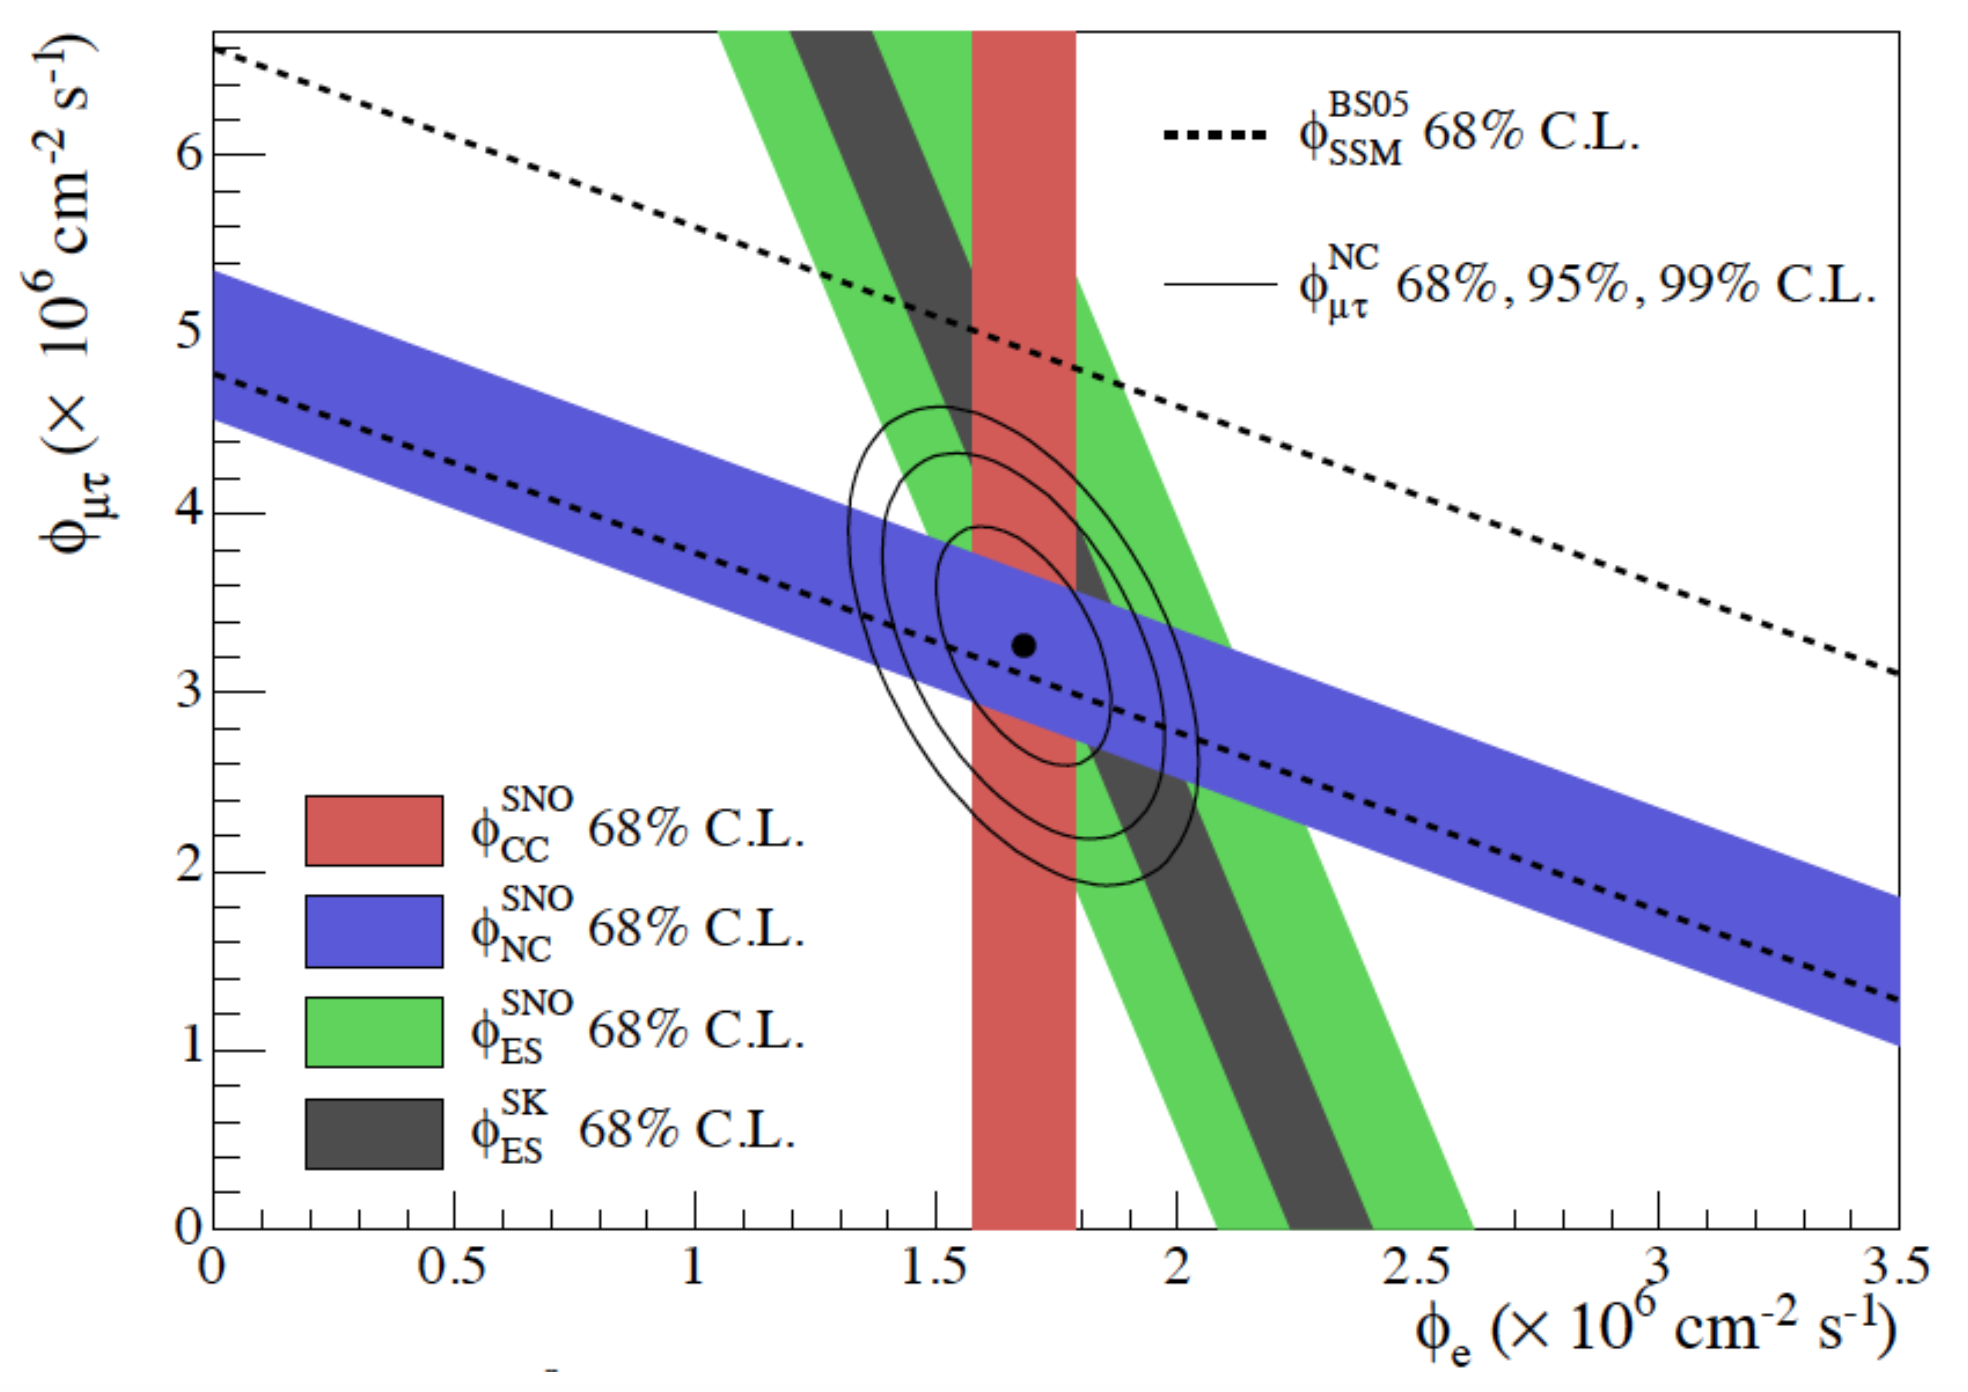
\includegraphics[width=0.6\textwidth]{Figures/sno.png}
\caption[Solar neutrino oscillation]{The flux of different scattering modes of solar neutrinos measured by SNO. The all-flavor flux (NC and ES) agreed. The day-night flux indicates $\nu_e$'s oscillation into other flavors. }
\label{fig:sno}
\end{figure}

\Section{Massive Neutrino}
    
    The discovery of neutrino oscillation implies massive neutrino.
    Although the natural origin of neutrino mass is undetermined, neutrinos can obtain mass through the Higgs mechanism similar to other leptons. 
    Under the assumption of neutrino being Dirac fermion (particle distinct from antiparticle), Higgs-lepton Yukawa Lagragian term can be written as
\begin{equation}\label{eq4}
\mathscr{L}_H = -\left(\frac{v+H}{\sqrt{2}}\right)\left[\overline{l'_L}Y'^{l}l'_R +\overline{\nu'_L}Y'^{\nu}\nu'_R\right],
\end{equation}
    where $v$ is the Higgs vacuum expectation value (VEV), $H$ is the higgs field, and $Y$ is the Yukawa coupling matrix. 
    The matrix can be diagonalized with the unitary matrice $V_L$ and $V_R$.
\begin{equation}\label{eq5}
V^\dagger_LY'V_R = Y,\   \ \textrm{with} \   \ Y_{kj} = y_k\delta_{kj} \   \ (k,j = 1,2,3),
\end{equation}
    where $y_k$ is the eigenvalue of Yukawa coupling matrix. The neutrino mass states array with the three-generation mixing is defined as:
\begin{equation}\label{eq6}
\nu'_L \rightarrow V^{\nu\dagger}_L\nu'_L = \left( \begin{array}{c}
\nu_{1L} \\
\nu_{2L} \\
\nu_{3L} \\
\end{array} \right) \   \ \text{and} \   \ \nu'_R \rightarrow V^{\nu\dagger}_R\nu'_R = \left( \begin{array}{c}
\nu_{1R} \\
\nu_{2R} \\
\nu_{3R} \\
\end{array} \right).
\end{equation}
    Consider $l_\alpha = l_{\alpha L} + l_{\alpha R}$ and $\nu_k = \nu_{kL} + \nu_{kR}$, the Lagrangian can be rewritten as
\begin{equation}\label{eq7}
\begin{aligned}
\mathscr{L}_H & = -\left(\frac{v+H}{\sqrt{2}}\right)\left[ \sum\limits_{\alpha = e, \mu, \tau} y_{\alpha}^l\overline{l_{\alpha L}}l_{\alpha R} + \sum\limits_{k = 1, 2, 3}y_k^\nu \overline{\nu_{kL}}\nu_{kR} \right] \\
& = - \sum\limits_{\alpha = e, \mu, \tau} \frac{y_\alpha^l v}{\sqrt{2}}\overline{l_{\alpha}}l_{\alpha} - \sum\limits_{k = 1, 2, 3} \frac{y_k^\nu v}{\sqrt{2}} \overline{\nu_{k}}\nu_{k} - \sum\limits_{\alpha = e, \mu, \tau} \frac{y_\alpha^l}{\sqrt{2}}\overline{l_{\alpha}}l_{\alpha}H - \sum\limits_{k = 1, 2, 3} \frac{y_k^\nu}{\sqrt{2}} \overline{\nu_{k}}\nu_{k}H.
\end{aligned}
\end{equation}
    Since $\nu_k = \nu_{kL} + \nu_{kR}$, the Dirac mass term of neutrino is simplified as
\begin{equation}\label{eq8}
\begin{aligned}
    \mathscr{L}^D_{mass} &= -\sum\limits_{k = 1, 2, 3} m_k^D\overline{\nu_{k}}\nu_{k} + \textrm{H.c.} \\
    & = -\sum\limits_{k = 1, 2, 3}m_k^D(\overline{\nu_{kL}}\nu_{kR} + \overline{\nu_{kR}}\nu_{kL}) + \textrm{H.c.},
\end{aligned}
\end{equation}
    where the Dirac mass of neutrino $m_k^D = \frac{y_k^\nu v}{\sqrt{2}}$ and $\overline{\nu_{kL}}\nu_{kL} = \overline{\nu_{kR}}\nu_{kR} = 0$.
    This mechanism for neutrino to obtain mass involves right handed neutrino $\nu_R$, also refered \textit{sterile neutrino} for its incapability of interacting under the parity violating weak force.
    
    Because of its neutral nature, neutrino is a candidate Majorana fermion (the particle is its own antiparticle).
    The 
    Under this condition, the neutrino field is
    \begin{equation}\label{eq9}
        \nu = \nu_L + \mathcal{C}\overline{\nu_L}^T,
    \end{equation}
    where neutrino $\mathcal{C}$ is charge conjugate matrix.
    The Majorana mass term of the lepton Lagrangian can be written as 
    \begin{equation}\label{eq10}
\begin{aligned}
    \mathscr{L}^M_{mass} &= \frac{1}{2}m_L{\nu_{L}^T} \mathcal{C}^\dagger \nu_{L} + \textrm{H.c.},
\end{aligned}
\end{equation}
    in which $m^L$ is the left handed Majorana mass.
    Majorana mass term of neutrino avoided the assumption of right handed neutrino.
    
    However, it is theoretically allowed that both right handed neutrino and Majorana neutrino can exist in theory. 
    Thus, a more general neutrino mass term for single neutrino scenario is defined as 
    \begin{equation}
    \label{eq11}
    \begin{aligned}
    \mathscr{L}_{mass}^{D+M} &= - m_D(\overline{\nu_{L}}\nu_{R} + \overline{\nu_{R}}\nu_{L}) + \frac{1}{2}m_L{\nu_{L}^T} \mathcal{C}^\dagger \nu_{L} + \frac{1}{2}m_R{\nu_{R}^T} \mathcal{C}^\dagger \nu_{R} + \textrm{H.c.} \\
    & = \frac{1}{2}(\begin{array}{cc}
    \overline{\nu^C_L} & \overline{\nu_R} \end{array}) 
    \left(\begin{array}{cc}
    m_L & m_D \\
    m_D & m_R
    \end{array}\right)
    \left(\begin{array}{c}
    \nu_L \\
    \nu_R^C
    \end{array}\right) + \textrm{H.c.}.
    \end{aligned}
    \end{equation}
    In a special case, when $m^D \ll m_R$ and $m_L = 0$, Equation~\ref{eq11} can be diagonalized as
    \begin{equation}
    \label{eq12}
    \mathscr{L}_{mass}^{D+M}  = \frac{1}{2}(\begin{array}{cc}
    \overline{\nu^1} & \overline{\nu_2} \end{array}) 
    \left(\begin{array}{cc}
    \frac{m_D^2}{m_R} &  \\
     & m_R
    \end{array}\right)
    \left(\begin{array}{c}
    \nu_1 \\
    \nu_2
    \end{array}\right) + \textrm{H.c.}
    \end{equation}
    This is called Type-I seesaw mechanism, a possible explanation of the tiny mass of left handed neutrino.

\Section{Theory of Neutrino Oscillation}
    
    The theoretical study of neutrino oscillation started in 1950s.
    Pontecorvo~\cite{bib:Pontecorvo1957, bib:Pontecorvo1957qd} proposed neutrino oscillation inspired from observation of $K^0 \leftrightarrow \overline{K}^0$ oscillation.
    In 1967, Maki, Nakagawa, and Sakata discussed the theory of two-neutrino fla mixing~\cite{bib:Maki1962}.
    Later in 1969, Gribov and Pontecorvo explicitly developed theory of neutrino oscillation with mass state mixing~\cite{bib:GRIBOV1969}. 
    By allowing massive neutrino, the neutrino portion of the Lagrangian can be expressed analogous to other massive particles.
\begin{equation}
\label{eq13}
\mathscr{L}_\nu = -\left[m^\nu_\alpha\overline{\nu_\alpha}\nu_\alpha + m^\nu_\beta\overline{\nu_\beta}\nu_\beta + m^\nu_\alpha m^\nu_\beta(\overline{\nu_\alpha}\nu_\beta + \overline{\nu_\beta}\nu_\alpha) \right] \   \ (\alpha, \beta = e, \mu, \tau).
\end{equation}
    This equation can be rewritten as
\begin{equation}
\label{eq14}
\mathscr{L}_\nu = \overline{\nu}_\alpha\mathcal{M}^\nu\nu_\beta.
\end{equation}
    where the $\mathcal{M}'^\nu$ is can be diagonalized. 
    The conversion between the two matrix expressions above transforms the flavor states of neutrino to mass states by a unitary matrix $U$:
\begin{equation}\label{eq15}
\left(\begin{array}{c}
\nu_\alpha \\
\nu_\beta
\end{array}\right) = \left(\begin{array}{cc}
\cos\theta & \sin\theta \\
-\sin\theta & \cos\theta
\end{array}\right)\left(\begin{array}{c}
\nu_k \\
\nu_l
\end{array}\right).
\end{equation}

    When $\theta \neq 0$, this transformation is a two generation mixing of neutrino mass eigenstates in the neutrino flavors, meaning neutrino's flavors are not orthogonal to its mass eigenstates.
    This matrix can be expanded to three neutrino mixing with the unitary matrix $U_{PMNS}$, the Pontecorvo-Maki-Nakagawa-Sakata (PMNS) matrix, a neutrino equivalent to the CKM mixing of quarks. 
    In addition to the 3x3 angle transformation, the matrix also includes the CP-violation phase factor $\delta_{CP}$ and a diagonal mixing matrix of Majorana neutrino term $D_\textrm{Majorana}$. 
    The three generation neutrino mixing matrix is 
    \begin{equation}\label{eq16}
    \begin{aligned}
    U & =  U_{PMNS}\cdot D_\textrm{Majorana} \\
    & =  \left(\begin{array}{ccc}
    U_{e1} & U_{e2} & U_{e3} \\
    U_{\mu 1} & U_{\mu 2} & U_{\mu 3} \\
    U_{\tau 1} & U_{\tau 2} & U_{\tau 3}
    \end{array}\right) \\
    & = \left(\begin{array}{ccc}
    1   &   &  \\
        &   c_{23}  & s_{23} \\
        &   -s_{23} & c_{23}
    \end{array}\right) 
    \left(\begin{array}{ccc}
    c_{13}  &   & s_{13}e^{-i\delta_{CP}} \\
        & 1 &  \\
    -s_{13}e^{i\delta_{CP}}  &   & c_{13}
    \end{array}\right) 
    \left(\begin{array}{ccc}
    c_{12}  & s_{12}  &  \\
    -s_{12} & c_{12} &  \\
        &   & 1
    \end{array}\right)  \\
    &\cdot\left( \begin{array}{ccc}
    e^{i\xi_1/2} & & \\
    & e^{-i\xi_1/2} & \\
    & & 1 \\
    \end{array}\right)
    \end{aligned}
    \end{equation}

    Hence, the flavor eigenstates of the neutrino can be described as a sum of the mass states with a matrix element form $U_{PMNS}$:
    \begin{equation}\label{eq17}
    |\nu_\alpha\rangle = \sum\limits_{k=1,2,3} U^*_{\alpha k}|\nu_k\rangle.
    \end{equation}
    Using the time-dependent Schr{\"o}dinger equation, the time evolution of neutrino flavor is expressed as
    \begin{equation}
    \label{eq18}
    |\nu_\alpha(t)\rangle = \sum\limits_{k=1,2,3} U^*_{\alpha k}e^{-i(E_k)t}|\nu_k\rangle.
    \end{equation}
    Therefore, the probability of a neutrino oscillating from one flavor to the other is
    \begin{equation}\label{eq19}
    \begin{aligned}
    P_{\nu_\alpha\rightarrow\nu_\beta} & =|\langle\nu_\beta|\nu_\alpha(t)\rangle|^2 \\
    & =\sum\limits_{k,j}U^*_{\alpha k} U_{\beta k} U_{\alpha j} U^*_{\beta j} e^{-i(E_k-E_j)t} \\
    & =\sum\limits_{k,j}U^*_{\alpha k} U_{\beta k} U_{\alpha j} U^*_{\beta j}\exp\left(-i\frac{\Delta m^2_{kj}L}{2E}\right),
    \end{aligned}
    \end{equation}
    where $\Delta m_{kj}^2 =m_k^2 - m_j^2$, $L$ is the neutrino travelling distance, and $E$ is the kinetic energy of neutrino.
    This equation proves a nonzero neutrino oscillation probability requires the mixing of massive neutrino.
    It also shows that the phase of the neutrino oscillation depends on the factor $\frac{\Delta m^2_{kj}L}{2E}$ explaining both the solar neutrino problem and the atmosphere neutrino anomaly. 
    
    The probability Equation~\ref{eq19} can be generalized to any neutrino flavor transition in oscillation as
\begin{equation}\label{eq20}
\begin{aligned}
	P_{\nu_\alpha\rightarrow\nu_\beta} = \delta_{\alpha\beta} & -  4 \sum\limits_{k>j}\textbf{Re} \left[ U^*_{\alpha k} U_{\beta k} U_{\alpha j} U^*_{\beta j}\right]\sin^2\left(\frac{\Delta m^2_{kj}L}{4E}\right) \\
	 & \pm 2 \sum\limits_{k>j} \textbf{Im} \left[
	 U^*_{\alpha k} U_{\beta k} U_{\alpha j} U^*_{\beta j}\right]\sin\left(-i\frac{\Delta m^2_{kj}L}{2E}\right).
\end{aligned}
\end{equation}
    The imaginary component is positive for neutrinos, and negative for antineutrinos. 
    In two neutrino mixing, Equation~\ref{eq19} can be simplified as
    \begin{equation}\label{eq21}
    \begin{aligned}
    P_{\nu_\alpha\rightarrow\nu_\beta} & = \sin^2{2\theta}\sin^2\left( 1.27\frac{\Delta m^2L}{E} \right)
    \end{aligned}
    \end{equation}
    to calculate the appearance probability of one flavor during neutrino oscillation in vacuum.
    Similarly, the survival probability of the original neutrino flavor can be written as 
    \begin{equation}\label{eq22}
    \begin{aligned}
    P_{\nu_\alpha\rightarrow\nu_\alpha} & = 1- \sin^2{2\theta}\sin^2\left( 1.27\frac{\Delta m^2L}{E} \right).
    \end{aligned}
    \end{equation}
    The probability equations (2.21) and (2.22) are frequently used as theoretical tool in neutrino oscillation experiments to calculate their oscillation models.

\Section{Measurements of Neutrino Oscillation}
    
    Experimental efforts have been made in the past two decades to determine the key neutrino oscillation parameters.
    By flux of survived and appeared neutrino during oscillation through varieties of baseline, the experiments is able to measure $\theta_{23}$, $\theta_{13}$, $\theta_{12}$, $\Delta m^2_{21}$ and $|\Delta m^2_{31}|$. 
    The $\theta_{12}$ and $\Delta m^2_{21}$ determined by the  phenomenological analyses of solar neutrino flux measurements~\cite{bib:SNOPRC} and KamLAND reactor \nuebar oscillation measurement~\cite{bib:KamLAND03}.
    By measuring the disappearance of $\nu_\mu$ and $\overline{\nu}_\mu$ in atmosphere neutrino experiments~\cite{bib:MACRO,bib:Soudan2}, long baseline accelerator neutrino experiments~\cite{bib:k2k,bib:MINOS,bib:t2k,bib:nova}, and neutrino telescope observation~\cite{bib:ANTARES, bib:ICEosc}, $\theta_{23}$ and $|\Delta m^2_{31(32)}|$ is measured.
    The $\theta_{13}$ is thoroughly measured through the short baseline reactor $\nuebar$ flux measurements~\cite{bib:DYBosc,bib:RENO,bib:DBChooz}, which is decribed in detail in Chapter~2.
    The results of the neutrino mass mixing parameters are shown in Table~\ref{tab:1.1}.
    \begin{table}[h]
    \centering
    \caption[Neutrino Oscillation Parameters]{Measured parameters of neutrino oscillation~\cite{bib:PDG}.}
    \begin{tabular}{lll}
    \hline
    \hline
    Parameters                  & Value             & 3-$\sigma$    \\ \hline
    $\sin^2(\theta _{12})$      & 0.297             & $0.250 - 0.354$
    \\ \hline
    $\sin^2(\theta _{23})$      & 0.425 (normal)    & $0.381 - 0.615$ \\
                                & 0.589 (inverted)  & $0.384 - 0.636$ \\ \hline
    $\sin^2(\theta_{13})$       & 0.0215 (normal)   & $0.0190 - 0.0240$ \\   
                                & 0.0216 (inverted) & $0.0190 - 0.0242$ \\ \hline
    $\Delta m^ 2_{21} (10^{-5}\textrm{eV}^2) $      & 7.57              & $6.93 - 7.96$ \\ \hline
    $|\Delta m^ 2_{31}| (10^{-3}\textrm{eV}^2) $    & 2.56 (normal)     & $2.45 - 2.69$\\
                                & 2.54 (inverted)   & $2.42 - 2.66$\\
    \hline
    \end{tabular}

    \label{tab:1.1}
    \end{table}
    
\Section{Future Tasks of Neutrino Experiments}
\label{ch1sec7}
    
    The properties of massive neutrino are of main interest of future experimental research, for it being the first solid experimental evidence of physics beyond standard model.
    
    The studies of Dirac or Majorana nature of neutrino are organized worldwide. 
    If neutrino less double $\beta$-decay ($0\nu\beta\beta$) is observed, neutrino can be determined as the first Majorana fermion ever detected.
    
    Several experiments are directly measuring the neutrino mass by searching for the end of $\beta$ spectrum with very high energy resolution. 
    
    The neutrino mass hierarchy, lepton CP violation and light sterile neutrino searching need more precise measurements of neutrino oscillation from different neutrino sources in different baselines. 
    These studies involve precise ratio of different transitions in oscillation, high resolution energy spectrum measurement, neutrino-antineutrino oscillation ratio, and very short baseline oscillation measurements.